%% This file was auto-generated by IPython.
%% Conversion from the original notebook file:
%% Exercise 8.ipynb
%%
\documentclass[11pt,english]{article}

%% This is the automatic preamble used by IPython.  Note that it does *not*
%% include a documentclass declaration. The documentclass is added at runtime
%% to the overall document.
\usepackage{fancyhdr}
\usepackage{amsmath}
\usepackage{amssymb}
\usepackage{graphicx}
\usepackage{ucs}
\usepackage[utf8x]{inputenc}

% needed for markdown enumerations to work
\usepackage{enumerate}

% Slightly bigger margins than the latex defaults
\usepackage{geometry}
\geometry{verbose,tmargin=3cm,bmargin=3cm,lmargin=2.5cm,rmargin=2.5cm}

% Define a few colors for use in code, links and cell shading
\usepackage{color}
\definecolor{orange}{cmyk}{0,0.4,0.8,0.2}
\definecolor{darkorange}{rgb}{.71,0.21,0.01}
\definecolor{darkgreen}{rgb}{.12,.54,.11}
\definecolor{myteal}{rgb}{.26, .44, .56}
\definecolor{gray}{gray}{0.45}
\definecolor{lightgray}{gray}{.95}
\definecolor{mediumgray}{gray}{.8}
\definecolor{inputbackground}{rgb}{.95, .95, .85}
\definecolor{outputbackground}{rgb}{.95, .95, .95}
\definecolor{traceback}{rgb}{1, .95, .95}

% Framed environments for code cells (inputs, outputs, errors, ...).  The
% various uses of \unskip (or not) at the end were fine-tuned by hand, so don't
% randomly change them unless you're sure of the effect it will have.
\usepackage{framed}

% remove extraneous vertical space in boxes
\setlength\fboxsep{0pt}

% codecell is the whole input+output set of blocks that a Code cell can
% generate.

% TODO: unfortunately, it seems that using a framed codecell environment breaks
% the ability of the frames inside of it to be broken across pages.  This
% causes at least the problem of having lots of empty space at the bottom of
% pages as new frames are moved to the next page, and if a single frame is too
% long to fit on a page, it will completely stop latex from compiling the
% document.  So unless we figure out a solution to this, we'll have to instead
% leave the codecell env. as empty.  I'm keeping the original codecell
% definition here (a thin vertical bar) for reference, in case we find a
% solution to the page break issue.

%% \newenvironment{codecell}{%
%%     \def\FrameCommand{\color{mediumgray} \vrule width 1pt \hspace{5pt}}%
%%    \MakeFramed{\vspace{-0.5em}}}
%%  {\unskip\endMakeFramed}

% For now, make this a no-op...
\newenvironment{codecell}{}

 \newenvironment{codeinput}{%
   \def\FrameCommand{\colorbox{inputbackground}}%
   \MakeFramed{\advance\hsize-\width \FrameRestore}}
 {\unskip\endMakeFramed}

\newenvironment{codeoutput}{%
   \def\FrameCommand{\colorbox{outputbackground}}%
   \vspace{-1.4em}
   \MakeFramed{\advance\hsize-\width \FrameRestore}}
 {\unskip\medskip\endMakeFramed}

\newenvironment{traceback}{%
   \def\FrameCommand{\colorbox{traceback}}%
   \MakeFramed{\advance\hsize-\width \FrameRestore}}
 {\endMakeFramed}

% Use and configure listings package for nicely formatted code
\usepackage{listingsutf8}
\lstset{
  language=python,
  inputencoding=utf8x,
  extendedchars=\true,
  aboveskip=\smallskipamount,
  belowskip=\smallskipamount,
  xleftmargin=2mm,
  breaklines=true,
  basicstyle=\small \ttfamily,
  showstringspaces=false,
  keywordstyle=\color{blue}\bfseries,
  commentstyle=\color{myteal},
  stringstyle=\color{darkgreen},
  identifierstyle=\color{darkorange},
  columns=fullflexible,  % tighter character kerning, like verb
}

% The hyperref package gives us a pdf with properly built
% internal navigation ('pdf bookmarks' for the table of contents,
% internal cross-reference links, web links for URLs, etc.)
\usepackage{hyperref}
\hypersetup{
  breaklinks=true,  % so long urls are correctly broken across lines
  colorlinks=true,
  urlcolor=blue,
  linkcolor=darkorange,
  citecolor=darkgreen,
  }

% hardcode size of all verbatim environments to be a bit smaller
\makeatletter
\g@addto@macro\@verbatim\small\topsep=0.5em\partopsep=0pt
\makeatother

% Prevent overflowing lines due to urls and other hard-to-break entities.
\sloppy

\newcommand{\HRule}{\rule{\linewidth}{0.5mm}}
\title{\bf Stochastic Optimization}
\author{Xugang Zhou \\ Fangzhou Yang}
\pagestyle{fancy}
\lhead{{\bf Machine Intelligence 2 SS2013}}
\rhead{Exercise 08}
\renewcommand{\headrulewidth}{0.4pt}

\begin{document}
\begin{titlepage}
\begin{center}
\vfill
\textsc{\LARGE Machine Intelligence 2}\\[1.5cm]
\textsc{\Large Exercise 08}\\[0.5cm]

\HRule \\[0.4cm]
{\huge \bfseries Stochastic Optimization}\\[0.4cm]
\HRule \\[1.5cm]
\begin{minipage}{0.4\textwidth}
\begin{flushleft} \large
\emph{Group Members:}\\
Xugang \textsc{Zhou}\\
Fangzhou \textsc{Yang}
\end{flushleft}
\end{minipage}
\begin{minipage}{0.4\textwidth}
\begin{flushright} \large
\emph{Tutor:} \\
Timm \textsc{Lochmann} \\
\end{flushright}
\end{minipage}
\vfill
{\large \today}\\
\end{center}
\end{titlepage}
\thispagestyle{fancy}

\section{8.1 Simulated Annealing}

\begin{codecell}
\begin{codeinput}
\begin{lstlisting}
from numpy import *
from math import *
import random

def E(w,s):
    tmp = 0.
    for i in range (len(s)):
        for j in range (len(s)):
            tmp += w[i,j] * s[i] * s[j]
    tmp = -tmp/2
    return tmp
def Esi(w,s,i):
    tmp = 0
    for j in range (len(s)):
        tmp += w[i,j] * s[i] * s[j]
    tmp = -tmp/2
    return tmp
def flip(s,deltaE,i,beta):
    if(beta*deltaE>100):
        p = 0
    else:
        p = (1. + math.exp(beta*deltaE) )**(-1)
    #print p, beta
    if (random.random()) < p:
        s[i] = -s[i]
        #print 'changed'
        
\end{lstlisting}
\end{codeinput}
\end{codecell}
\begin{codecell}
\begin{codeinput}
\begin{lstlisting}
#Initialization
beta0 = 0.001
tao =1.01
tmax = 1000
random.seed(100)
N = 6
Et = [ 0. for i in range(tmax)]
beta = [0. for i in range(tmax)]
beta[0] = beta0

S = [0 for i in range (N)]
for i in range(N):
    if(random.random()>0.5):
        S[i] = 1
    else:
        S[i] = -1
W = matrix([[0. for i in range(N)]for j in range (N)])
for i in range(N):
    for j in range(N):
        if(i==j): W[i,j] =0
        if(i<j): W[i,j] = random.random()
        if(i>j): W[i,j] = W[j,i]
print 'beta0:', beta0
print 'tao:',tao
print 'tmax:',tmax
print 'W:'
print W
print 'S', S
\end{lstlisting}
\end{codeinput}
\begin{codeoutput}
\begin{verbatim}
beta0: 0.001
tao: 1.01
tmax: 1000
W:
[[ 0.          0.80002046  0.53290141  0.08015371  0.45594588  0.04788752]
 [ 0.80002046  0.          0.9329624   0.94707801  0.33535078  0.30940593]
 [ 0.53290141  0.9329624   0.          0.76801815  0.20386953  0.17846076]
 [ 0.08015371  0.94707801  0.76801815  0.          0.18859491  0.34700445]
 [ 0.45594588  0.33535078  0.20386953  0.18859491  0.          0.62632164]
 [ 0.04788752  0.30940593  0.17846076  0.34700445  0.62632164  0.        ]]
S [-1, -1, 1, 1, 1, -1]
\end{verbatim}
\end{codeoutput}
\end{codecell}
\begin{codecell}
\begin{codeinput}
\begin{lstlisting}
#optimization
for t in range(tmax):
    i = random.randint(0,5)
    Et[t] = E(W,S)
    localE = Esi(W,S,i)
    deltaE = -2 * localE
    flip(S,deltaE,i,beta[t]) 
    if((t+1) < tmax):
        beta[t+1] = tao*beta[t]

\end{lstlisting}
\end{codeinput}
\end{codecell}
\begin{codecell}
\begin{codeinput}
\begin{lstlisting}
#plotting
import matplotlib
import matplotlib.pyplot as plt


Tt = [ 1/beta[t] for t in range (tmax)]

fig = plt.figure()
ax = fig.add_subplot(111)
ax.plot(Tt)
ax.set_title("Temperature")
plt.show()

fig = plt.figure()
ax = fig.add_subplot(111)
ax.plot(Et)
ax.set_title("Energy")
plt.show()

print S
\end{lstlisting}
\end{codeinput}
\begin{codeoutput}
\begin{center}
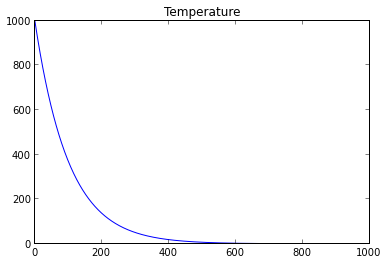
\includegraphics[width=0.7\textwidth]{Exercise_8_files/Exercise_8_fig_00.png}
\par
\end{center}
\begin{center}
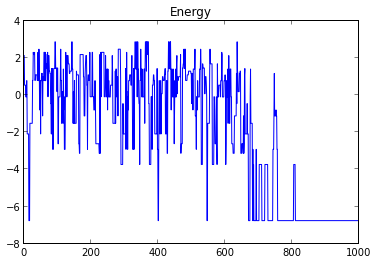
\includegraphics[width=0.7\textwidth]{Exercise_8_files/Exercise_8_fig_01.png}
\par
\end{center}
\begin{verbatim}
[-1, -1, -1, -1, -1, -1]
\end{verbatim}
\end{codeoutput}
\end{codecell}
\begin{codecell}
\begin{codeinput}
\begin{lstlisting}
m = [0 for i in range(6)]
S_all = [[0 for p in range(6)] for q in range(64)]
tmp = 0
E_all = [0 for i in range(64)]
for m[0] in range(2):
    for m[1] in range(2):
        for m[2] in range(2):
            for m[3] in range(2):
                for m[4] in range(2):
                    for m[5] in range(2):
                        for i in range(6):
                            if(m[i] == 0):
                                S_all[tmp][i] = -1
                            else:
                                S_all[tmp][i] = 1
                        E_all[tmp] = E(W,S_all[tmp])
                        tmp = tmp +1

ind = np.arange(64)
fig = plt.figure()
ax = fig.add_subplot(111)
ax.bar(ind, E_all)
plt.show()
                        
\end{lstlisting}
\end{codeinput}
\begin{codeoutput}
\begin{center}
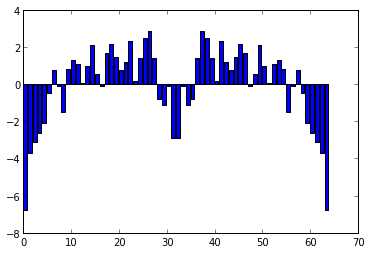
\includegraphics[width=0.7\textwidth]{Exercise_8_files/Exercise_8_fig_02.png}
\par
\end{center}
\end{codeoutput}
\end{codecell}
\begin{codecell}
\begin{codeinput}
\begin{lstlisting}
Z = 0

beta = [0.01, 0.1, 0.5, 1]

P = [[0 for i in range(64)] for j in range(len(beta))]

for m in range (len(beta)):
    for i in range (64):
        Z += math.exp(-beta[m]*E(W,S_all[i]) )
    for i in range (64):
        P[m][i] = math.exp(-beta[m]*E(W,S_all[i]))/Z
    
    ind = np.arange(64)
    fig = plt.figure()
    ax = fig.add_subplot(111)
    ax.set_title('beta:'+ (str)(beta[m]))
    ax.bar(ind, P[m])
    plt.show()

\end{lstlisting}
\end{codeinput}
\begin{codeoutput}
\begin{center}
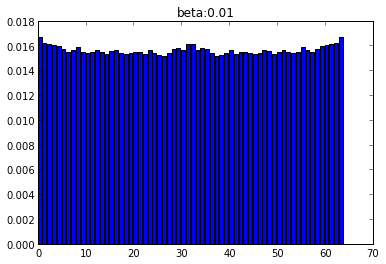
\includegraphics[width=0.7\textwidth]{Exercise_8_files/Exercise_8_fig_03.png}
\par
\end{center}
\begin{center}
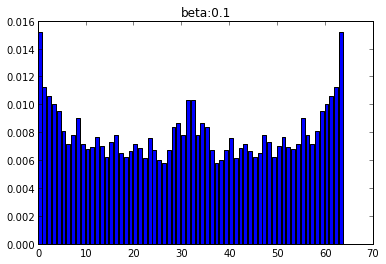
\includegraphics[width=0.7\textwidth]{Exercise_8_files/Exercise_8_fig_04.png}
\par
\end{center}
\begin{center}
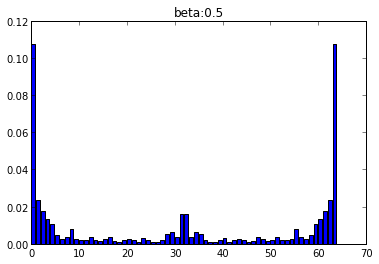
\includegraphics[width=0.7\textwidth]{Exercise_8_files/Exercise_8_fig_05.png}
\par
\end{center}
\begin{center}
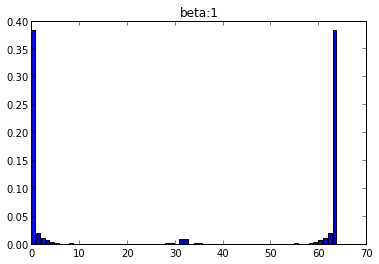
\includegraphics[width=0.7\textwidth]{Exercise_8_files/Exercise_8_fig_06.png}
\par
\end{center}
\end{codeoutput}
\end{codecell}
\section{8.2 Mean-Field Annealing}

\begin{codecell}
\begin{codeinput}
\begin{lstlisting}
def e(w,s,i):
    tmp = 0.
    for j in range(len(s)):
        tmp = w[i,j] * s[j]
    return tmp

def et(w,s):
    tmp = 0.
    for i in range(len(s)):
        for j in range(len(s)):
           tmp += w[i,j] * s[i] * s[j]
    tmp = -0.5 * tmp
    return tmp
\end{lstlisting}
\end{codeinput}
\end{codecell}
\begin{codecell}
\begin{codeinput}
\begin{lstlisting}
#Initialization
beta0 = 0.001
tao =1.01
tmax = 1000
random.seed(100)
N = 6
Et = [ 0. for i in range(tmax)]
beta = [0. for i in range(tmax)]
beta[0] = beta0

S = [0 for i in range (N)]
for i in range(N):
    S[i] = random.random()*2-1
    W = matrix([[0. for i in range(N)]for j in range (N)])
for i in range(N):
    for j in range(N):
        if(i==j): W[i,j] =0
        if(i<j): W[i,j] = random.random()
        if(i>j): W[i,j] = W[j,i]
print 'beta0:', beta0
print 'tao:',tao
print 'tmax:',tmax
print 'W:'
print W
print 'S', S

\end{lstlisting}
\end{codeinput}
\begin{codeoutput}
\begin{verbatim}
beta0: 0.001
tao: 1.01
tmax: 1000
W:
[[ 0.          0.80002046  0.53290141  0.08015371  0.45594588  0.04788752]
 [ 0.80002046  0.          0.9329624   0.94707801  0.33535078  0.30940593]
 [ 0.53290141  0.9329624   0.          0.76801815  0.20386953  0.17846076]
 [ 0.08015371  0.94707801  0.76801815  0.          0.18859491  0.34700445]
 [ 0.45594588  0.33535078  0.20386953  0.18859491  0.          0.62632164]
 [ 0.04788752  0.30940593  0.17846076  0.34700445  0.62632164  0.        ]]
S [-0.7086614897917394, -0.0901459909719573, 0.5415676113180443, 0.4110264538680559, 0.4639179460665115, -0.1329711302091925]
\end{verbatim}
\end{codeoutput}
\end{codecell}
\begin{codecell}
\begin{codeinput}
\begin{lstlisting}
#optimization
for t in range(tmax):
    i = random.randint(0,5)
    ei = e(W,S,i)
    Et[t]= et(W,S)
    S[i] = math.tanh(beta[t]*ei)
    if((t+1)<tmax):
        beta[t+1] = tao * beta[t]
        
        
\end{lstlisting}
\end{codeinput}
\end{codecell}
\begin{codecell}
\begin{codeinput}
\begin{lstlisting}
#plotting

Tt = [ 1/beta[t] for t in range (tmax)]

fig = plt.figure()
ax = fig.add_subplot(111)
ax.plot(Tt)
ax.set_title("Temperature")
plt.show()

fig = plt.figure()
ax = fig.add_subplot(111)
ax.plot(Et)
ax.set_title("Energy")
plt.show()

print S

\end{lstlisting}
\end{codeinput}
\begin{codeoutput}
\begin{center}
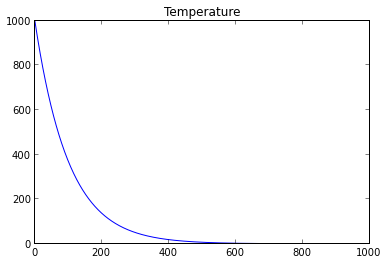
\includegraphics[width=0.7\textwidth]{Exercise_8_files/Exercise_8_fig_07.png}
\par
\end{center}
\begin{center}
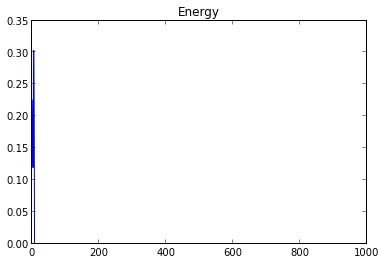
\includegraphics[width=0.7\textwidth]{Exercise_8_files/Exercise_8_fig_08.png}
\par
\end{center}
\begin{verbatim}
[-0.0, -0.0, -0.0, -0.0, -0.0, -0.0]
\end{verbatim}
\end{codeoutput}
\end{codecell}

\end{document}
